\section{Distribution of Potential and Kinetic Energy of Bound Particles after a Finite Time}
\label{sec:DistributionPotKinEnBound}
The virial theorem states the following relation for the kinetic energy $E_{kin}$ and potential energy $E_{pot}$ of a bound gravitational system in equilibrium. 
\begin{align}
	2\left< E_{kin} \right> = - \left< E_{pot} \right>
	\label{eq:ViralTheorem}
\end{align}
$\left< E_{kin} \right>$ and $\left< E_{pot} \right>$ represents the time average of the kinetic and potential energy, respectively, but by the ergodic hypothesis, this can be made the ensamble average \cite{Project5_CompPhys}. 

To study whether the virial theorem of \matref{eq:ViralTheorem} is fulfilled with the computed algorithms, the final kinetic and potential energy of the bound particles of a system initially consisting of 70 particles after a time period of $\tau_{crunch}$.
It is expected that the fraction of the mean of the kinetic energy and the mean of the potential energy will be close to $-2$, even though it in \secref{sec:StabilityAndEquilibrium} is found that the equilibrium is not reached before than after a time period of $2\tau_{crunch}$. 

In addition, to get rid of some of the numerical instabilities, a smoothing function, as argued for in \secref{sec:argumentforepsilon}, is introduced.
To check the consistency with the virial theorem of the fourth order Runge-Kutta method when including the smoothing function, similar histograms for the distribution of the kinetic energy and potential energy after a finite time period as shown in \figref{fig:DistributionPotKinEnBoundHistograms} is generated to determine the mean of the kinetic energy and potential energy.
The bound particles are found by the same argument as in \secref{sec:EnergyRK4} that a particle is bound if the total energy of that particle is negative, that is the particle is bound if the absolute value of the potential energy is greater than the absolute value of the kinetic energy.
\begin{figure}[H]
\centering
\begin{minipage}{.5\textwidth}
  \centering
  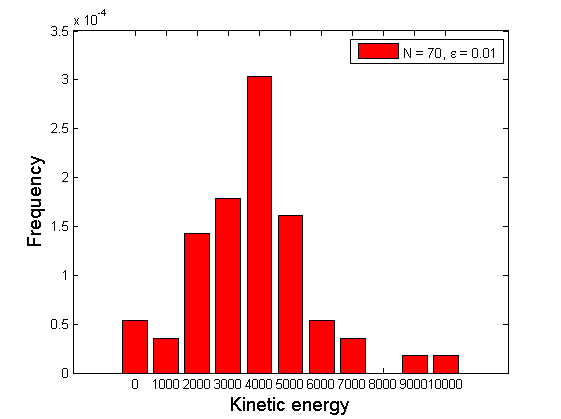
\includegraphics[width=1\linewidth]{Figures/Histograms_including_epsilon/N_70_e_n3_kin.png}
\end{minipage}%
\begin{minipage}{.5\textwidth}
  \centering
  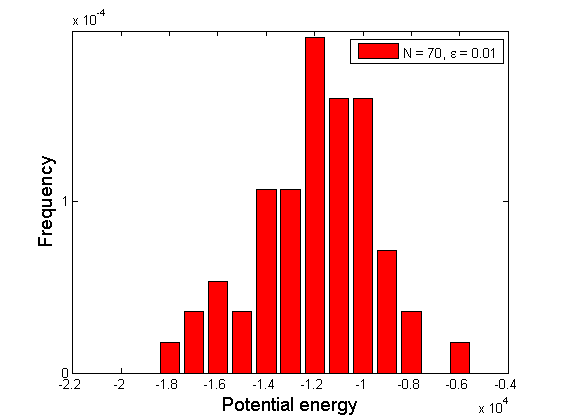
\includegraphics[width=1\linewidth]{Figures/Histograms_including_epsilon/N_70_e_n3_pot.png}
\end{minipage}
\caption{
	Distribution of the kinetic and potential energy of bound particles in the star cluster after a time period of $1\tau_{crunch}$ with a step length of $1\times 10^{-4} \tau_{crunch}$ and $\epsilon = 1\times 10^{-2} \text{ ly}$ for 70 particles with normal distributed masses, uniformly distributed within a sphere generated by the functions presented in \secref{Method:GeneratingPosMassVel}. 
}
\label{fig:DistributionPotKinEnBoundHistograms}
\end{figure}
The kinetic and the potential energy of the bound particles seem to follow a more or less uniform distribution after a finite time period. 
This is also seen when computing histograms for different values of $\epsilon$. 
The mean of these distributions for the kinetic energy and potential energy after are shown in the table below for various values of $\epsilon$. 

\begin{table}[H]
\centering
\begin{tabular}{|c|c|c|c|c|}
\hline
$\epsilon$ (ly)  & $\left< E_{kin} \right>$ & $\left< E_{pot} \right>$ & $\left< E_{pot} \right>$/$\left< E_{kin} \right>$ \\
\hline
0 & 952.0 & -2409 & -2.53	
\\ \hline
0.1 & 4036 & -7886 & -1.95
\\ \hline
$10^{-2}$ & 1119 & -2846 & -2.54
\\ \hline
$10^{-3}$ & 2548 & -4860 & -1.91
\\ \hline
$10^{-4}$ & 2531 & -4489 & -1.77
\\ \hline
$10^{-5}$ & 2129 & -3677 & -1.73
\\ \hline
$10^{-6}$ & 567.5 & -1774 & -3.13
\\ \hline
$10^{-7}$ & 1333 & -2444 & -1.83
\\ \hline
$10^{-8}$ & 1368 & -2635 & -1.93
\\ \hline
\end{tabular}
\caption{
Mean of kinetic energy and potential energy for bound particles after a time period of $3\tau_{crunch}$ with a step length of $10^{-4} \tau_{crunch}$ for a star cluster with initially 70 particles uniformly distributed in a sphere of radius $20\text{R}_{\odot}$.
The computed potential energy is divided by two, since in the computation the potential energy is doubled when summing up for all particles. 
}
\label{tab:DistributionPotKinEnBound}
\end{table}
From \tabref{tab:DistributionPotKinEnBound} it is seen that for no values of $\epsilon$, the virial theorem is fulfilled. 
However, the fraction $\left< E_{pot} \right>$/$\left< E_{kin} \right>$ approaches the value $-2$, when $\epsilon$ is introduced for all values except $\epsilon = 10^{-6}$.
The fraction of the energies is in the figure below plotted as a function of $\epsilon$, and it is seen from the figure, as well from \tabref{tab:DistributionPotKinEnBound} that most of the choices of $\epsilon$ will be an improvement of the result compared having $\epsilon = 0$, according to the virial theorem.
Since $10^{-7} \text{ly}$ corresponds to $1.36\text{R}_{\odot}$ this is chosen as the optimal $\epsilon$, due to the fact that is has the physical meaning of being similar to what one can expect the radius of the considered particles to be.
\begin{figure}[H]
\centering
	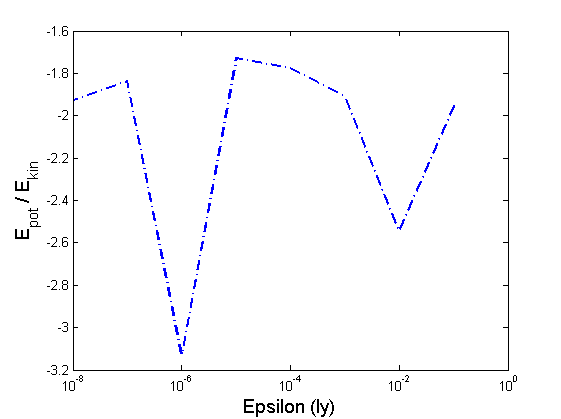
\includegraphics[width=0.6\linewidth]{Figures/epsilon_frac.png}
\caption{
The value of the energy fraction $\left< E_{pot} \right>$/$\left< E_{kin} \right>$, that according to the virial theorem should equal $-2$, as a function of $\epsilon$ introduced in \matref{eq:SmoothingFct}.
}
\label{fig:epsilonfrac}
\end{figure}
The histograms in \figref{fig:DistributionPotKinEnBoundHistograms2} below show the distribution of the kinetic energy and potential energy of the bound particles after a time period of $3\tau_{crunch}$, hence after reached equilibrium. 
The distribution of the energies of the bound particles seems no longer to be Gaussian as was seen for a time period of $1\tau_{crunch}$ in \figref{fig:DistributionPotKinEnBoundHistograms}.
\begin{figure}[H]
\centering
\begin{minipage}{.5\textwidth}
  \centering
  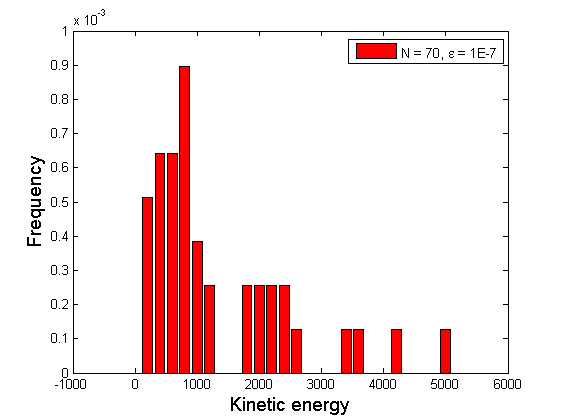
\includegraphics[width=1\linewidth]{Figures/epsilon7_kin.png}
\end{minipage}%
\begin{minipage}{.5\textwidth}
  \centering
  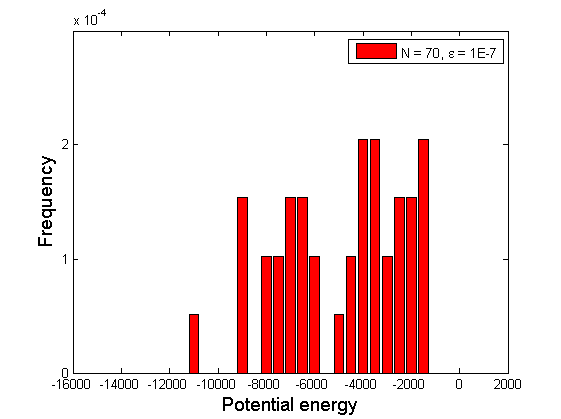
\includegraphics[width=1\linewidth]{Figures/epsilon7_pot.png}
\end{minipage}
\caption{
	Distribution of the kinetic and potential energy of bound particles in the star cluster after a time period of $1\tau_{crunch}$ with a step length of $1\times 10^{-4} \tau_{crunch}$ and $\epsilon = 1\times 10^{-2} \text{ ly}$ for 70 particles with normal distributed masses, uniformly distributed within a sphere generated by the functions presented in \secref{Method:GeneratingPosMassVel}. 
}
\label{fig:DistributionPotKinEnBoundHistograms2}
\end{figure}